\chapter{Постановка задачи}
Целью  данной работы является создание маршевого (безытерационного) вычислительного алгоритма для решения задачи переноса излучения на неструктурированных трехмерных сетках. 

Основными задачами, решаемыми в данной работе, являются:
\begin{itemize}
\item Разработка алгоритма упорядочения - основа маршевого метода
\item Разработка метода повышенного порядка аппроксимации
\item Сравнение результатов, полученных различными методами.
\end{itemize}

В работе \cite{skalko_2014} приведен алгоритм упорядочения, но он предазначен исключительно для триангуляций, удовлетворяющих условию Делоне. При разработке метода повышенного порядка аппроксимации неизбежно возникает проблема обеспечения <<физичности>> решения, которую можно обеспечить при монотонности используемой схемы.
\section{Математическая модель}
Поле излучения, заполняющего пространство, описывается распределением интенсивности излучения по частотам, в пространстве и по направлениям переноса лучистой энергии. Пусть $f(\nu, \vec r, \vec \Omega, t)d\nu d\vec r d \vec \Omega \, $ есть число световых квантов в спектральном интервале от $ \nu$ до $ \nu + d\nu$, находящихся в момент $t$ в элементе объема $d\vec r$ около точки $\vec r$ и имеющих направление движения в элементе телесного угла $d\vec \Omega$ около единичного вектора $\vec \Omega$. 
Каждый квант обладает энергией $h \nu$ и движется со скоростью $c$, поэтому величина 
\begin {equation}
I_{\nu} (\vec r, \vec \Omega, t)d \nu d\vec \Omega = h\nu c f (\nu, \vec r, \vec \Omega, t)d\nu d\vec{\Omega}
\end {equation}
есть количество лучистой энергии в спектральном интервале $d\nu$, протекающей в $1 \text{ сек}$ через площадку в $1 \text{ см}^2$, помещенную в точке $\vec r$ перпендикулярно к направлениям распространения энергии, которые лежат в элементе телесного угла $d\vec\Omega$ около вектора $\vec \Omega$. Задание функций $I_{\nu}$ или $f$ полностью определяет поле излучения. Количество лучистой энергии, заключенной  спектральном интервале $d\nu$ и находящейся в $1 \text{ см}^3$ пространства в точке $\vec r$ в момент $t$, или спектральная плотность излучения, равно:
\begin {equation}
U_\nu (\vec r, t) = h \nu \int_{4 \pi} f d \Omega = \frac{1}{c} \int_{4\pi} I_{\nu} d\Omega.
\end {equation}

Вектор спектрального потока равен 
\begin {equation}
\vec S_{\nu} = \int_{4\pi} I_{\nu}\vec\Omega d\Omega,
\end {equation}
где $\vec\Omega$ - единичный вектор направления движения квантов. 
Полные интенсивность, плотность и поток излучения получаются из спектральных интегрированием их по всему спектру частот:
\begin {equation}
I = \int_0^\infty I_{\nu} d\nu, \quad U = \int_0^\infty U_{\nu}d\nu, \quad \vec S =  \int_0^\infty \vec S_{\nu}d\nu.
\end {equation}
\section{Уравнение переноса}
Рассмотрим баланс излучения в элементарном цилиндре \ref{fig:1} с площадью основания $d\sigma$ и высотой $ds$, расположенном в данной точке пространства таким образом, что направление $\vec\Omega$ совпадает с образующей цилиндра и перпендикулярно к его основаниям. За время $dt$ в левое основание втекает количество излучения $I_{\nu} (\vec\Omega, \vec r,t)d\sigma dt$. Из правого основания за тот же промежуток времени вытекает количество излучения $(I_{\nu} + dI_{\nu})d \sigma dt$.

\begin{figure}[ht!]
\centering{
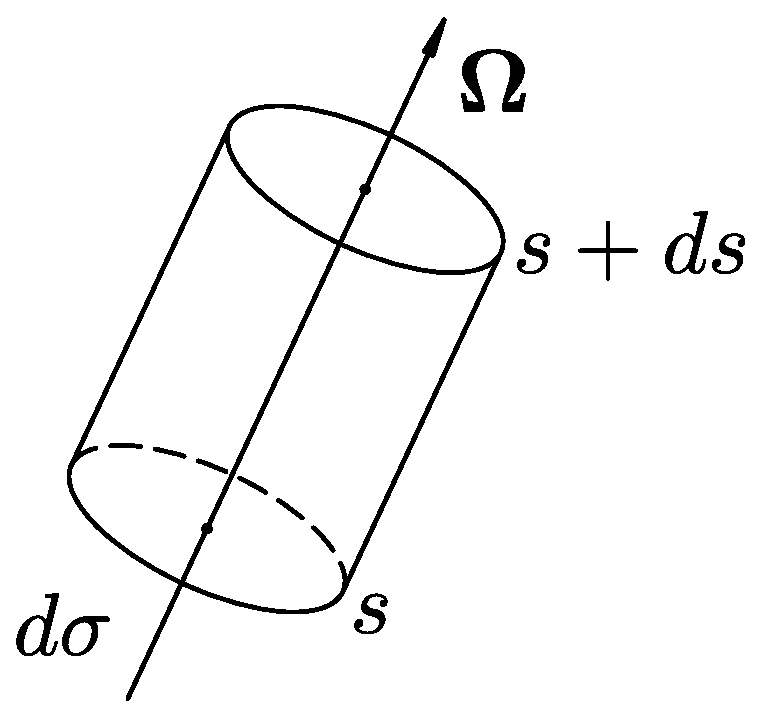
\includegraphics[width = 0.3\textwidth]{cylinder.eps}
}
\caption{К выводу уравнения переноса излучения}
\label{fig:1}
\end{figure}

Интенсивность $I_{\nu}$ есть функция координат и времени. Приращение интенсивности пучка света при переходе от левого основания к правому складывается из локального приращения за время прохождения светом пути $ds$ и из приращения при переходе от координаты $s$ к координате $s+ds$ в данный момент времени, 
\begin {equation}
dI_{\nu}  = \frac{\partial I_{\nu}}{\partial t } \frac{ds}{c}+\frac{\partial I_{\nu}}{\partial s}ds.
\end {equation}

Введем коэффициент поглощения $\varkappa_\nu$ таким образом, что количество лучистой энергии в интервале частот $d\nu$ и интервале направлений $d\vec\Omega$, поглощаемой в $1 \text{ см}^3$ в  $1 \text{ сек}$, равно
\begin {equation}
I_{\nu}d\nu d\vec\Omega \varkappa_{\nu}.
\label {3}
\end {equation}
Обозначим плотность самопроизвольного испускания $j_\nu$. То есть количество энергии, самопроизвольно испускаемой веществом  в $1 \text{ см}^3$ в  $1 \text{ сек}$ интервале $d\nu d\vec\Omega$, равно $j_{\nu}d\nu d\vec\Omega$. Помимо самопроизвольного испускания также существует так называемое вынужденное испускание. Вероятность вынужденного испускания кванта данной частоты и данного направления пропорциональна имеющейся в данной точке пространства интенсивности излучения той же частоты и того же направления. Известно \cite{zeld_2013}, что полная вероятность испускания данных квантов пропорциональна величине $1+n$, где $n = c^2I_{\nu}/2h\nu^3$. Таким образом, полное количество излучения, испускаемого в $1 \text{ сек}$ в $1 \text{ см}^3$ в интервале $d\nu d\vec\Omega$, равно 
\begin {equation}
j_{\nu} d\nu d\vec\Omega \left(1+\frac{c^2}{2h\nu^3}I_{\nu}\right).
\label{4}
\end {equation}
Первое слагаемое в скобках соответствует спонтанному испусканию, а второе - вынужденному. 

Количество излучения, испущенного в цилиндре за время $dt$, согласно формуле \eqref{4}, равно
\begin {equation}
j_{\nu}\left(1 + \frac {c^2}{2h\nu^3}I_{\nu}\right)d\sigma ds dt.
\end {equation}
Поглощается в нем за то же время количество излучения $\varkappa_{\nu} I_{\nu}d\sigma dsdt$. Составляя баланс и поделив полученное выражение на произведение дифференциалов $d\sigma dsdt$, получим уравнение
\begin {equation}
\frac{1}{c} \left(\frac{\partial I_{\nu}}{\partial t} + c \vec \Omega \nabla I_{\nu}\right) = j_{\nu} \left(1 + \frac {c^2}{2h\nu^3}I_{\nu}\right) - \varkappa_{\nu}I_{\nu}.
\label{1}
\end {equation}

Преобразуем правую часть уравнения \eqref{1}, объединив вместе члены, отвечающие поглощению и вынужденному испусканию, поскольку они оба пропорциональны неизвестной функции координат и времени - интенсивности излучения. 

Рассмотрим среду, находящуюся в состоянии термодинамического равновесия при постоянной температуре $T$. В стационарных условиях поле излучения также равновесно. Спектральная функция плотности равновесного излучения $U_{\nu p}$ подчиняется закону Планка. Количество энергии равновесного излучения частоты $\nu$ в $1 \text{ см}^3$, приходящееся на единичный интервал частот, равно
\begin {equation}
U_{\nu p} = \frac{8 \pi h \nu^3}{c^3} \frac {1}{e^{\frac{h\nu}{kT}} - 1}
\end {equation}
В силу изотропии спектральная интенсивность равновесного излучения равна
\begin {equation}
I_{\nu p} = \frac{cU_{\nu p}}{4\pi} = \frac{2h\nu^3}{c^2}\frac{1}{e^{\frac{h\nu}{kT}} - 1}
\label{5}
\end {equation}

В состоянии термодинамического равновесия испускание и поглощение квантов данных частоты и направления в точности компенсируют друг друга, так что выражения \eqref{3} и \eqref{4} следует приравнять, причем интенсивность излучения $I_{\nu}$ заменить при этом равновесной величиной $I_{\nu p}$. 
Принимая во внимание формулу \eqref{5} для равновесной интенсивности, найдем, что отношение лучеиспускательной способности любого вещества к его коэффициенту поглощения есть универсальная функция частоты и температуры:
\begin {equation}
\frac{j_{\nu}}{\varkappa_{\nu}} =  \frac{I_{\nu p}}{1+\frac{c^2}{2h\nu^3}I_{\nu p}} = \frac{2h\nu^3}{c^2}e^{-\frac{h\nu}{kT}}.
\label{6}
\end {equation}

Это отношение представляет собой одну из форм закона Кирхгофа. Формулу \eqref{6} удобно переписать в виде
\begin {equation}
j_{\nu} = I_{\nu p}\varkappa_{\nu}\left(1-e^{-\frac{h\nu}{kT}}\right).
\label{7}
\end {equation}

В новой трактовке закон Кирхгофа \eqref{7} приобретает форму
\begin {equation}
j_{\nu} = \varkappa'_{\nu}I_{\nu p}, \quad \varkappa'_{\nu} = \varkappa_{\nu}\left(1 - e^{-\frac{h\nu}{kT}}\right).
\end {equation}

Введем при этом в множитель перед $I_{\nu}$ в члене вынужденного испускания вместо коэффициента излучения $j_{\nu}$ его выражение через коэффициент поглощения, в которое подставим формулу \eqref{5} для равновесной интенсивности. Правая часть уравнения \eqref{1} примет вид 
\begin {equation}
j_{\nu} - \varkappa_{\nu}\left(1 - e^{-\frac{h\nu}{kT}}\right)I_{\nu}.
\end {equation}
Отсюда видно, что вынужденное испускание можно трактовать как некое уменьшение поглощения: часть квантов поглощается и тут же испускается снова с той же частотой и в том же направлении, причем вероятность этого <<переизлучения>> равна $e^{-\frac{h\nu}{kT}}$. Можно считать, что коэффициент поглощения имеет несколько меньшую величину:
\begin {equation}
\varkappa'_{\nu} = \varkappa_{\nu}\left(1 - e^{-\frac{h\nu}{kT}}\right).
\end {equation}

Взаимодействие излучения с веществом можно представлять так, как будто существует только спонтанное испускание и эффективное поглощение, описываемое коэффициентом $\varkappa'_{\nu}$, исправленным на вынужденное испускание. 

Вводя это выражение в правую часть уравнения переноса \eqref{1} запишем уравнение в следующей форме:
\begin {equation}
\frac{1}{c}\frac{\partial I_{\nu}}{\partial t} + (\vec\Omega \nabla) I_{\nu} = \varkappa'_{\nu} (I_{\nu p} - I_{\nu}).
\label{2}
\end {equation}

Будем в дальнейшем понимать под $\varkappa_\nu$ коэффициент поглощения $\varkappa_\nu'$, т.е. подправленный на спонтанное излучение.
\section {Граничные условия}
Дополним уравнение \eqref{2} граничными условиями \cite{chetv_1985}. Они должны определять только излучение, приходящее извне в исследуемый объем. Мы ограничиваемся случаем заданного излучения извне, поскольку условия отражения связывают уравнения переноса в разных направлениях. В случае выпуклых областей для направлений $\vec\Omega$, выходящих в рассматриваемую область, имеет место неравенство $(\vec\Omega, \vec n) < 0$, где $\vec n$ -- вектор внешней нормали к границе $G$ (см рис \ref{fig:6}).
\begin{figure}[ht!]
	\centering{
		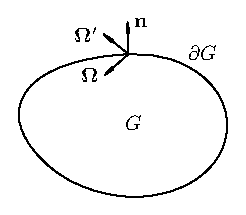
\includegraphics[width = 0.4\textwidth]{bord.eps}
	}
	\caption{Граничные условия для выпуклых областей. На участке границы $\partial G$ происходит зеркальное отражение фотонов}
	\label{fig:6}
\end{figure}

Граничное условие на границе $G$ примет вид
\begin {equation}
I_\nu (G, \vec\Omega, \nu, t) = I_\nu^*(G, \vec\Omega, \nu, t), \quad (\vec\Omega, \vec n) < 0.
\end {equation}
Здесь $I_\nu^*$ - известная функция, определяющая приходящее извне излучение. В работе используется граничное условие вида
\begin {equation}
I_\nu (G, \vec\Omega, \nu, t) = 0, \quad (\vec\Omega, \vec n) < 0.
\end {equation}
Это условие соответствует тому, что источники излучения находятся только внутри рассматриваемой области.

Иногда часть границы области $\partial G$ отражает выходящее из объема излучение. Простейшим случаем отражения является зеркальное отражение. При этом отражение происходит по законам классической оптики:
\begin {equation}
I_\nu (G, \vec\Omega, \nu, t) = \delta I_\nu(\partial G, \vec\Omega_1, \nu, t), 
\end {equation}
где $\vec\Omega_1 = \vec\Omega - 2\vec n( \vec\Omega\vec n)$ --- симметричное к $\vec\Omega$ относительно нормали $\vec n$ направление, $\delta$ --- коэффициент отражения, $0 \leqslant \delta \leqslant 1$.
\section{Аналитическое решение уравнения переноса}
Найдем формальное решение уравнения переноса излучения, рассматривая величины, зависящие только от состояния вещества $I_{\nu p}(T)$, $\varkappa_{\nu}(T, \rho)$, как известные функции координат и времени. Рассмотрим сначала для простоты стационарный случай, когда распределения температуры и плотности, а также поле излучения не зависят от времени. Будем интересоваться излучением в точке $\vec r$ тела с направлением распространения $\vec \Omega$ (см. рис. \ref{fig:2}). 
\begin{figure}[ht!]
\centering{
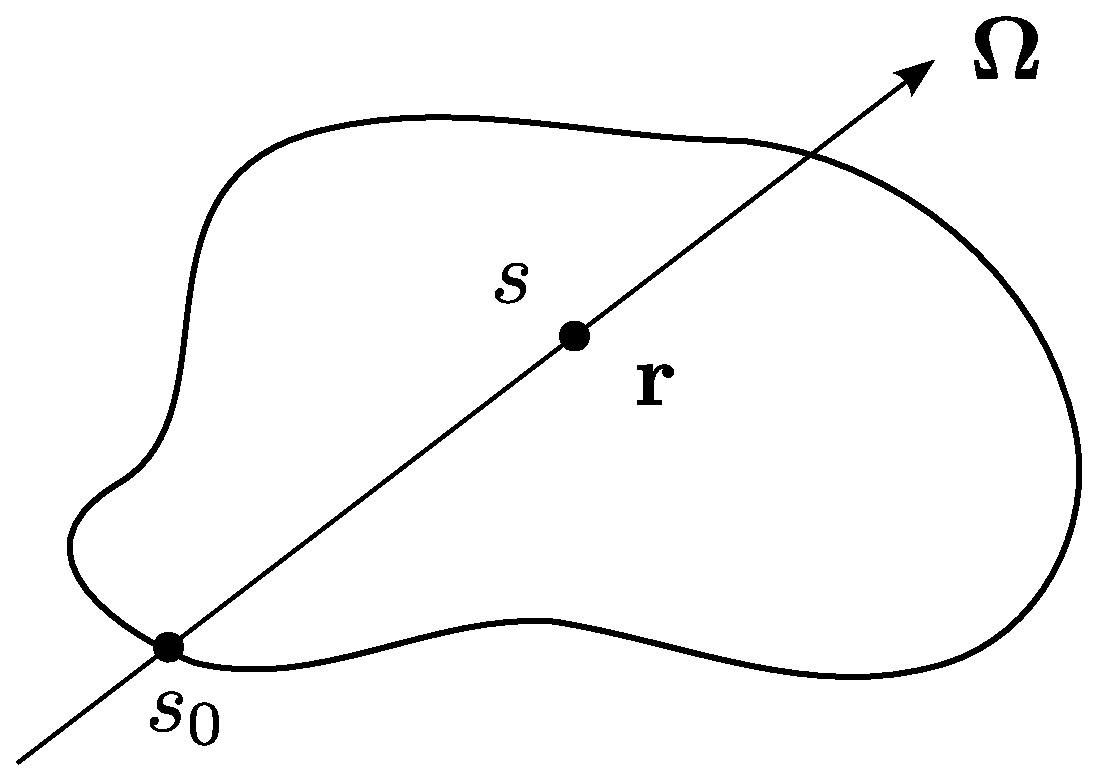
\includegraphics[width = 0.4\textwidth]{analytic.eps}
}
\caption{Схема, поясняющая пределы интегрирования в формуле для точного решения}
\label{fig:2}
\end{figure}
Проведем луч через данную точку в данном направлении и обозначим координату вдоль луча через $s$. Замечая, что дифференциальное выражение в левой части уравнения переноса \eqref{2} представляет собой полную производную от интенсивности вдоль луча распространения, перепишем уравнение в виде
\begin {equation}
\frac{dI_{\nu}}{ds} + \varkappa_{\nu}I_{\nu} = \varkappa_{\nu}I_{\nu p}.
\end {equation}
Это уравнение можно рассматривать как обыкновенное линейное уравнение относительно интенсивности вдоль луча. Решение его есть:
\begin {equation}
I_{\nu}(s) = \int_{s_0}^s\varkappa_{\nu}I_{\nu p} \exp\Big[-\int_{s'}^s\varkappa_{\nu}ds''\Big]ds' + I_{\nu,0} \exp\Big[-\int_{s_0}^s \varkappa_{\nu}ds''\Big].
\label{8}
\end {equation}

Здесь $I_{\nu}(s)$ - интенсивность $I_{\nu}(\vec r, \vec\Omega)$, которая рассматривается как функция координаты $s$ вдоль луча. Интегрирование по лучу ведется от границы тела $s_0$ (как показано на \ref{fig:2}). Через $I_{\nu, 0}$ обозначена константа интегрирования, которая имеет смысл значения интенсивности излучения на границе в точке $s_0$.

Величина
\begin{equation}
\tau(s_1, s_2) = \int_{s_1}^{s_2} \varkappa_\nu ds
\end{equation}
называется оптической толщиной вдоль луча от точки $s_1$ до точки $s_2$. Будем называть область от $s_1$ до $s_2$ оптически плотной, если $\tau(s_1, s_2) \gg 1$ и оптически прозрачной, если $\tau(s_1, s_2) \ll 1$.
С использованием оптической толщины формула \eqref{8} для интенсивности в точке $s$ может быть записана в виде
\begin{equation}
I_\nu(s) = \int_{s_0}^s \varkappa_\nu I_{\nu p} e^{-\tau(s', s)} ds'
+ I_{\nu,0} e^{-\tau(s_0, s)}
.
\label{eq:8_5}
\end{equation}